\documentclass[11pt,letterpaper]{article}

\usepackage[utf8]{inputenc}
\usepackage[T1]{fontenc}
\usepackage[spanish,mexico]{babel}
\usepackage[margin=2.5cm]{geometry}
\usepackage{enumitem}
\usepackage{graphicx}
\usepackage{xcolor}
\usepackage{booktabs}
\usepackage[hidelinks]{hyperref}
\usepackage{fancyhdr}
\usepackage{titlesec}

\definecolor{guinda}{RGB}{122,30,58}

\titleformat{\section}{\normalfont\Large\bfseries\color{guinda}}{\thesection}{1em}{}
\titleformat{\subsection}{\normalfont\large\bfseries}{\thesubsection}{1em}{}

\pagestyle{fancy}
\fancyhf{}
\fancyhead[L]{\small Práctica 2 — Bases de Datos}
\fancyhead[R]{\small ESCOM-IPN}
\fancyfoot[C]{\thepage}
\renewcommand{\headrulewidth}{0.4pt}

\begin{document}

\begin{titlepage}
\centering
\vspace*{2cm}

{\Large\bfseries INSTITUTO POLITÉCNICO NACIONAL\par}
\vspace{0.4cm}
{\large ESCUELA SUPERIOR DE CÓMPUTO\par}

\vspace{2.5cm}

{\color{guinda}\rule{\textwidth}{1.5pt}}
\vspace{0.6cm}

{\Huge\bfseries Requisitos ampliados\par}
\vspace{0.4cm}
{\LARGE Gestor académico ESCOM\par}
\vspace{0.3cm}
{\large Modelo Entidad-Relación Extendido --- Proyecto propio\par}

\vspace{0.6cm}
{\color{guinda}\rule{\textwidth}{1.5pt}}

\vspace{2.5cm}

\begin{tabular}{rl}
\textbf{Unidad de aprendizaje:} & Bases de Datos \\[0.3em]
\textbf{Programa académico:} & Ingeniería en Sistemas Computacionales \\[0.3em]
\textbf{Plan de estudios:} & 2020 \\[0.3em]
\textbf{Práctica:} & 2 --- Modelo EER \\[0.3em]
\textbf{Ejercicio:} & 4 --- Modelo EER del proyecto propio \\[0.3em]
\textbf{Equipo:} & Catscoms \\
\end{tabular}

\vfill
{\large Septiembre 2026\par}
\end{titlepage}

\tableofcontents
\newpage

\section{Origen del proyecto}

Este proyecto no partió de un supuesto: surgió de un problema que uno de los integrantes del equipo vivió directamente. A mitad de semestre, al notar que varias materias iban mal encaminadas, apareció una pregunta concreta que resultó sorprendentemente difícil de responder: \textit{¿qué voy a poder inscribir el próximo semestre?}

Responderla implicaba cruzar información dispersa en al menos cuatro lugares distintos: el kardex para saber qué materias se habían reprobado, el estado del alumno para conocer la situación académica (regular o irregular) y cuántas materias permitía inscribir, el módulo de horarios de SAES para ver qué grupos se abrían y en qué bloques, y sitios externos como MisProfesores para decidir con qué profesor intentar de nuevo una materia ya reprobada. Ninguno de esos cuatro lugares habla con los otros, y ninguno muestra el panorama completo: cuál sería un horario viable, sin choques, que respete el tope de materias, que incluya los recursos pendientes y que además evite a los profesores con peores evaluaciones.

De esa necesidad nació una primera versión funcional del sistema, desarrollada como aplicación web sin backend, disponible en:

\begin{center}
\url{https://github.com/staywildamond-gif/iscweb}
\end{center}

Esa versión resolvió el problema inmediato --- permitía capturar el avance personal, ver métricas de profesores y armar un horario automático sin choques --- pero lo hizo con datos estáticos en archivos JavaScript y estado guardado en \texttt{localStorage} del navegador. Funciona para un estudiante en una sola computadora, y ahí se acaba: no hay forma de que varios estudiantes lo usen, de conservar el histórico de varios periodos, de que las evaluaciones de profesores se alimenten de la comunidad, ni de que la información sobreviva a limpiar la caché del navegador.

\subsection{Objetivo de esta etapa}

El objetivo de esta etapa es rediseñar ese sistema sobre una base de datos relacional real con backend, de modo que deje de ser una herramienta personal y se convierta en un gestor académico utilizable por cualquier estudiante de ESCOM, en cualquiera de sus tres carreras. Este documento presenta los requisitos ampliados y el modelo entidad-relación extendido que sustentan ese rediseño.

\section{Descripción del problema}

Los estudiantes de ESCOM-IPN (ISC, IIA y LCD) planean cada reinscripción de forma manual, consultando fuentes que no se comunican entre sí:

\begin{itemize}[nosep]
  \item El módulo de horarios de SAES (\url{https://www.saes.escom.ipn.mx/Academica/horarios.aspx}), para conocer los grupos que se abren.
  \item El kardex (\url{https://www.saes.escom.ipn.mx/Alumnos/boleta/kardex.aspx}), para saber qué materias se aprobaron y cuáles se reprobaron.
  \item El estado del alumno (\url{https://www.saes.escom.ipn.mx/Alumnos/boleta/Estado_Alumno.aspx}), que determina si la situación es regular o irregular y cuántas materias se permiten inscribir.
  \item Sitios externos de evaluación de profesores, como MisProfesores.
  \item El calendario académico oficial del IPN, revisado por separado de la agenda personal de tareas y exámenes.
\end{itemize}

No existe un sistema que centralice esta información período a período, que cubra las tres carreras con la misma estructura, que combine el calendario oficial con recordatorios personales, ni que use las calificaciones de los propios compañeros para decidir qué grupo tomar.

El sistema propuesto es un gestor y agenda académica, disponible como aplicación web con posibilidad de empaquetarse como aplicación instalable, que centraliza por período académico y por carrera: el catálogo de materias del plan de estudios vigente (con su liga oficial al PDF del programa), los grupos que se abren cada período con su cupo, turno y profesor, las calificaciones que los estudiantes dan a los profesores, el horario personal que cada estudiante arma para inscribirse, el calendario oficial de actividades del IPN, y una agenda personal donde el estudiante agrega sus propios eventos y tareas.

\section{Alcance multiusuario y multi-carrera}

El sistema es multiusuario: cada estudiante tiene su propia cuenta, pertenece a una de las tres carreras de ESCOM (ISC, IIA, LCD), y tiene su propio avance de materias cursadas y aprobadas, así como su propio horario armado por período. Las tres carreras comparten la misma estructura de datos (plan de estudios, grupos, ramas de especialización); solo cambia el contenido específico de cada una. Las reseñas de profesores son visibles para todos los estudiantes, pero cada reseña pertenece a quien la escribió. El calendario oficial del IPN es el mismo para las tres carreras; la agenda personal es privada de cada estudiante.

Cada estudiante tiene además una \textbf{situación escolar} que cambia período a período, equivalente a lo que SAES muestra en el módulo de estado del alumno. No es un valor binario entre regular e irregular: el procedimiento oficial de reinscripción distingue al menos seis categorías (cero adeudos; uno o más adeudos sin dictamen ni desfase; unidad de aprendizaje desfasada; dictamen vigente del CGC o del CTCE; regreso de baja temporal; recuperado de ETS especial), y cada una determina una carga y una ocupabilidad distintas. El historial completo de materias cursadas y sus calificaciones --- lo que en SAES corresponde al kardex --- se obtiene directamente del conjunto de registros históricos de la relación \textbf{Cursa} a través de todos los períodos, sin necesidad de una entidad aparte.

\section{Reglas de carga académica y situación escolar}

El procedimiento de reinscripción de ESCOM no se rige por un simple máximo de materias, sino por un sistema de \textbf{cargas} medidas en unidades de aprendizaje (UA) y por la \textbf{situación escolar} del estudiante en ese período. El modelo debe reproducir estas reglas:

\subsection{Cargas por programa académico}

\begin{center}
\begin{tabular}{lcc}
\toprule
\textbf{Programa académico} & \textbf{Carga mínima (UA)} & \textbf{Carga media (UA)} \\
\midrule
ISC 2020 & 4 & 7 \\
IIA 2020 & 4 & 6 \\
LCD 2020 & 4 & 6 \\
\bottomrule
\end{tabular}
\end{center}

Las unidades de aprendizaje \textbf{adeudadas se contabilizan dentro de la carga}: un estudiante con adeudos no suma materias nuevas sobre su carga normal, sino que sus adeudos ocupan lugares de la misma cuota. Además, Trabajo Terminal I y Trabajo Terminal II equivalen a dos unidades de aprendizaje cada una, por lo que el modelo guarda el valor en UA como atributo propio de cada materia y no asume que toda materia valga uno.

\subsection{Ocupabilidad según situación escolar}

La \textbf{ocupabilidad} --- el número de lugares a los que el estudiante puede aspirar --- no es un atributo del grupo, sino que depende de la situación escolar del estudiante en ese período:

\begin{center}
\begin{tabular}{lcc}
\toprule
\textbf{Situación escolar} & \textbf{Carga} & \textbf{Ocupabilidad} \\
\midrule
Cero adeudos & Hasta carga media & 30 \\
Uno o más adeudos, sin dictamen ni desfase & Hasta carga media & 34 \\
Unidad de aprendizaje desfasada & Según situación & 36 \\
Dictamen vigente CGC o CTCE & Según situación & 36 \\
Regreso de baja temporal & Según situación & 36 \\
Recuperado de ETS especial & Según situación & 36 \\
\bottomrule
\end{tabular}
\end{center}

Esta es la razón por la que el modelo introduce la entidad débil \textbf{InscripcionPeriodo}: la situación escolar, la ocupabilidad y la carga permitida no son propiedades permanentes del estudiante ni del grupo, sino de la combinación estudiante--período. Un mismo estudiante puede ser regular un semestre e irregular al siguiente, y su ocupabilidad cambia con él.

\subsection{Prioridad de adeudos}

Un estudiante irregular no puede inscribir libremente: sus materias adeudadas tienen prioridad y consumen cuota antes que cualquier materia nueva. Conforme recursa y aprueba esos adeudos, su situación escolar mejora y su cuota disponible se recalcula. El sistema modela esto con el atributo \texttt{es\_adeudo} en la relación \textbf{Cursa}, lo que permite distinguir en cada inscripción qué materias son recursos obligatorios y cuáles son avance nuevo. En la aplicación, esta regla se traduce en un bloqueo con advertencia: el sistema impide armar un horario que omita adeudos pendientes, pero permite al estudiante continuar bajo su propia responsabilidad si decide ignorar la recomendación.

\subsection{Otras restricciones de cardinalidad}

\begin{itemize}
  \item Todo grupo tiene exactamente un profesor titular asignado; un profesor puede tener cero o varios grupos en un período.
  \item Todo grupo imparte exactamente una materia; una materia puede tener varios grupos por período o ninguno.
  \item Toda materia optativa pertenece a exactamente una rama de especialización; toda rama agrupa al menos una materia optativa. Cursar optativas es obligatorio, pero el estudiante elige libremente en qué rama hacerlo según su interés.
  \item Cada inscripción concreta a un grupo (\textbf{Cursa}) admite a lo sumo una reseña, lo que garantiza que solo reseña quien efectivamente cursó y que nadie reseñe dos veces el mismo curso.
  \item El Artículo 98 del Reglamento Interno del IPN establece que ningún alumno puede cursar unidades de aprendizaje correspondientes a más de tres períodos escolares consecutivos, ni adeudar las de más de dos períodos previos al que cursa. El modelo puede verificar ambas reglas recorriendo el historial de \textbf{Cursa} por período.
\end{itemize}

\section{Prerrequisitos del mapa curricular}

El plan de estudios define qué unidades de aprendizaje deben aprobarse antes de cursar otras. Esto se modela como una \textbf{relación recursiva} sobre \textbf{Materia}: una materia requiere cero o más materias previas, y a su vez habilita cero o más materias posteriores. En la notación Crow's Feet esta relación se resuelve con la tabla asociativa \textbf{Prerrequisito}, cuya clave primaria compuesta evita duplicados y permite representar grafos de dependencias de cualquier profundidad.

\section{Entidades que dependen de otras}

\begin{itemize}
  \item \textbf{Grupo} no existe sin un \textbf{Periodo}: el mismo código de grupo (por ejemplo \texttt{6CV3}) se reutiliza en distintos períodos, así que su identidad completa depende de a qué período pertenece. Es dependencia de \textbf{identificación}.
  \item \textbf{SesionHorario} no existe sin un \textbf{Grupo}: es el bloque día/hora que ocupa ese grupo; si el grupo se cancela, sus sesiones dejan de tener sentido. Es dependencia de \textbf{existencia}.
  \item \textbf{EventoPersonal} no existe sin un \textbf{Estudiante}: un recordatorio o tarea carece de sentido fuera de la cuenta que lo creó. Es dependencia de \textbf{existencia}.
  \item \textbf{InscripcionPeriodo} no existe sin un \textbf{Estudiante} y un \textbf{Periodo}: es el registro de la situación escolar, ocupabilidad y carga de ese estudiante en ese semestre concreto. Es dependencia de \textbf{identificación}: su clave es precisamente la combinación de ambos.
  \item \textbf{ReporteResena} no existe sin una \textbf{Resena}: es el señalamiento de una reseña presuntamente abusiva. Es dependencia de \textbf{existencia}.
\end{itemize}

\section{Categorías dentro de entidades principales}

\textbf{Materia} se divide en dos tipos con comportamiento distinto:

\begin{itemize}[nosep]
  \item \textbf{MateriaObligatoria}: pertenece a un semestre fijo del plan y puede tener grupos de recurse.
  \item \textbf{MateriaOptativa}: pertenece a una rama de especialización y se cursa en un slot fijo (A1, B1, A2 o B2).
\end{itemize}

Esta división es \textbf{total} (toda materia cae en una de las dos) y \textbf{disjunta} (ninguna materia es de ambos tipos a la vez), porque el plan de estudios ISC-2020 así las distingue desde el catálogo oficial.

\section{Relaciones que involucran más de dos entidades}

La reseña de un profesor no tiene sentido sin especificar en qué grupo y período fue evaluado: el mismo profesor puede impartir la misma materia en distintos grupos con desempeño distinto. Por eso \textbf{Reseña} es una relación ternaria entre \textbf{Estudiante}, \textbf{Profesor} y \textbf{Grupo} (que lleva el período implícito), no una relación binaria simple.

\section{Sistema de reseñas de la comunidad}

Los sistemas previos con objetivos similares tomaban las métricas de profesores de fuentes externas, lo que los volvía dependientes de datos que no controlaban y que no reflejaban necesariamente la experiencia del grupo. Este proyecto conserva un import inicial de esas métricas como punto de partida, pero incorpora un sistema propio de reseñas escritas por los estudiantes bajo las mismas métricas ya establecidas: calidad, dificultad y porcentaje de recomendación, más un texto libre de hasta 400 caracteres.

Tres decisiones de modelado sostienen este sistema:

\begin{enumerate}
  \item \textbf{Anonimato opcional.} Cada reseña lleva el atributo \texttt{es\_anonima}. La autoría siempre se registra en la base de datos --- es lo que permite verificar y moderar --- pero la aplicación oculta el nombre del autor cuando así se solicita.

  \item \textbf{Verificación por agregación.} Una reseña no se asocia directamente al par (estudiante, profesor), sino a un registro concreto de \textbf{Cursa}: la inscripción verificada de ese estudiante en ese grupo. Esto constituye una \textbf{agregación}: la relación Cursa se trata como una entidad de orden superior que participa en la relación Resena. De ahí se derivan dos garantías: solo puede reseñar quien efectivamente cursó con ese profesor en ese grupo, y nadie puede reseñar dos veces el mismo curso.

  \item \textbf{Moderación.} La entidad débil \textbf{ReporteResena} registra los señalamientos de contenido abusivo, con su motivo, quién reportó y el estado de resolución, lo que permite retirar reseñas sin borrar el historial de la moderación.
\end{enumerate}

\section{Calendario oficial y agenda personal}

El calendario académico del IPN (inscripción, periodo de evaluaciones, vacaciones, días de descanso obligatorio) se modela como una entidad independiente ligada al período escolar: son fechas iguales para todos los estudiantes de las tres carreras. Sobre esa base, cada estudiante puede agregar su propia agenda personal (tareas, recordatorios, exámenes propios), que opcionalmente puede asociarse a una materia específica. El calendario oficial es la fuente principal y de solo lectura; la agenda personal es un complemento editable por cada estudiante.

\section{Recursos por materia}

Cada materia del plan de estudios incluye una liga al PDF oficial de su programa, tal como los publica ESCOM. Por ejemplo, la ficha de Matemáticas Discretas del plan ISC-2020:

\begin{center}
\small\url{https://www.escom.ipn.mx/docs/oferta/uaISC2020/matematicasDiscretas_ISC2020.pdf}
\end{center}

Este dato se guarda como atributo simple de la materia, no como entidad aparte, porque por ahora se contempla un único recurso oficial por materia.

\section{Preguntas que responde el sistema}

\begin{enumerate}[nosep]
  \item ¿Qué grupos de una materia tienen cupo disponible en el período actual, en cualquiera de las tres carreras?
  \item ¿Qué profesor tiene mejor calificación promedio para una materia específica, considerando solo reseñas de estudiantes que la cursaron realmente?
  \item ¿Cómo ha cambiado la ocupación de una materia (cupo contra inscritos) a lo largo de los últimos periodos?
  \item ¿Qué materias optativas de una rama concreta se han ofrecido, y en qué slot, dentro de una carrera?
  \item ¿Qué estudiantes tienen una materia bloqueada por haberla reprobado dos veces?
  \item ¿Qué eventos oficiales del calendario caen dentro de los próximos quince días, combinados con las tareas personales del estudiante?
\end{enumerate}

\section{Justificación de las entidades débiles}

\textbf{Grupo} no puede existir de forma independiente porque su identidad real no es solo el código (\texttt{6CV3}), sino ese código \textit{dentro de un período específico}: ESCOM reabre los mismos códigos de grupo cada semestre, así que dos grupos \texttt{6CV3} de periodos distintos son entidades completamente distintas, con distinto profesor, distinto cupo y distintos inscritos. Sin la dependencia de identificación hacia \textbf{Periodo} sería imposible distinguirlos con una sola clave, y el historial académico mezclaría inscripciones de semestres diferentes como si fueran la misma.

\textbf{SesionHorario} no puede existir de forma independiente porque un bloque de día y hora solo tiene sentido como parte del horario de un grupo concreto: si el grupo se cancela o cambia de horario, esa sesión deja de tener referente. Es dependencia de existencia y no de identificación, porque una sesión sí podría identificarse por sus propios atributos (día más bloque), pero jamás aparece sin que exista antes su grupo.

\textbf{EventoPersonal} es igualmente de existencia: si se elimina la cuenta del estudiante, sus eventos personales pierden todo propósito.

\section{Justificación de la especialización elegida}

Se eligió que \textbf{Materia} se especialice en \textbf{MateriaObligatoria} y \textbf{MateriaOptativa} con restricción \textbf{disjunta y total} porque así es exactamente como el plan de estudios ISC-2020 --- y previsiblemente los de IIA y LCD --- clasifica cada materia desde el catálogo oficial: no existe una materia que sea ambas cosas a la vez (disjunta), y toda materia del plan cae en una de las dos categorías, sin materias sueltas sin clasificar (total).

Una especialización parcial habría implicado que el sistema permitiera materias sin tipo, lo cual generaría inconsistencias al momento de armar el horario: no se sabría si aplica el flujo de recurse (propio de las obligatorias) o el flujo de slot de rama (propio de las optativas).

\section{Cómo las cardinalidades reflejan las reglas de negocio}

\begin{itemize}
  \item \textbf{Cursa (InscripcionPeriodo--Grupo) (0,carga\_media):(0,cupo).} El límite superior del lado del estudiante no es una constante del modelo, sino el valor de \texttt{carga\_media} de su carrera (7 UA en ISC, 6 en IIA y LCD), contabilizando los adeudos. Ligar la cardinalidad a un atributo de \textbf{Carrera} y no a un número fijo permite que las tres carreras convivan en el mismo esquema sin reglas duplicadas.
  \item \textbf{Registra (Estudiante--InscripcionPeriodo) (0,N):(1,1) y EnPeriodo (1,1):(0,N).} Estas cardinalidades son las que hacen posible el histórico: cada semestre genera un registro independiente con su propia situación escolar y ocupabilidad, en vez de sobrescribir un único estado del estudiante.
  \item \textbf{Imparte (Profesor--Grupo) (0,N):(1,1).} Ningún grupo puede impartirse sin profesor asignado, de ahí el (1,1) del lado del grupo; pero un profesor puede no tener grupos ese período (licencia, año sabático), de ahí el (0,N) de su lado.
  \item \textbf{Agrupa (Rama--MateriaOptativa) (1,N):(1,1).} Obliga a que toda materia optativa tenga una rama definida, sin quedar huérfana, pero no obliga a que un estudiante elija una rama específica: esa libertad de elección vive en la relación \textbf{Cursa}, no en \textbf{Agrupa}.
\end{itemize}

\section{Tres consultas que un modelo sin conceptos extendidos no podría resolver}

\begin{enumerate}
  \item \textbf{¿Cuántos estudiantes están inscritos en el grupo \texttt{6CV3} del período 2025-2, y cuántos en el \texttt{6CV3} del período 2026-1?} Solo es posible distinguirlos porque \textbf{Grupo} es una entidad débil identificada por \textbf{Periodo}. Un modelo donde el código de grupo fuera clave primaria por sí solo mezclaría ambos periodos en un mismo registro.

  \item \textbf{Lista de materias optativas de una rama concreta, en la carrera ISC, que además tienen grupos de recurse disponibles.} Requiere la jerarquía de especialización para filtrar solo \texttt{MateriaOptativa} con su rama, cruzándolo con la partición por carrera. Sin la especialización, el atributo de recurse (propio de obligatorias) y los de slot y rama (propios de optativas) tendrían que convivir como columnas opcionales sueltas en una sola tabla, sin garantía de que no se mezclen indebidamente.

  \item \textbf{Calificación promedio que los estudiantes dieron a un profesor específicamente en un grupo y período dados, contando solo reseñas verificadas de quienes realmente lo cursaron.} Depende de la \textbf{agregación}: \textbf{Reseña} no se ancla al par (estudiante, profesor), sino a un registro concreto de \textbf{Cursa}, tratado como entidad de orden superior. Sin ese mecanismo no habría forma de distinguir una reseña legítima de una escrita por alguien que nunca tomó la clase, ni de diferenciar el desempeño del mismo profesor entre grupos o periodos.

  \item \textbf{Qué materias puede inscribir un estudiante el próximo período, dados sus adeudos, su ocupabilidad y los prerrequisitos que ya aprobó.} Esta es la pregunta que originó el proyecto, y requiere tres conceptos extendidos a la vez: la entidad débil \textbf{InscripcionPeriodo} para conocer su situación escolar y cuota de ese semestre, la relación recursiva \textbf{Prerrequisito} para saber qué materias están desbloqueadas, y el atributo \texttt{es\_adeudo} sobre \textbf{Cursa} para dar prioridad a lo reprobado. Un modelo plano, sin entidades débiles ni relaciones recursivas, tendría que resolver esto fuera de la base de datos.
\end{enumerate}

\section{Herramienta utilizada para los diagramas}

Los diagramas de ambas notaciones se generaron con \textbf{Graphviz}, describiendo el modelo en lenguaje DOT. Se eligió esta herramienta porque el diagrama queda definido en un archivo de texto plano, lo que permite versionarlo en el repositorio junto con el resto del proyecto, revisar los cambios del modelo en el historial de Git como cualquier otro código, y regenerar las imágenes de forma reproducible cada vez que el modelo cambia, sin depender de un editor gráfico ni de un servicio externo.

\section{Diagramas del modelo}

\subsection{Notación de Peter Chen}

\begin{center}
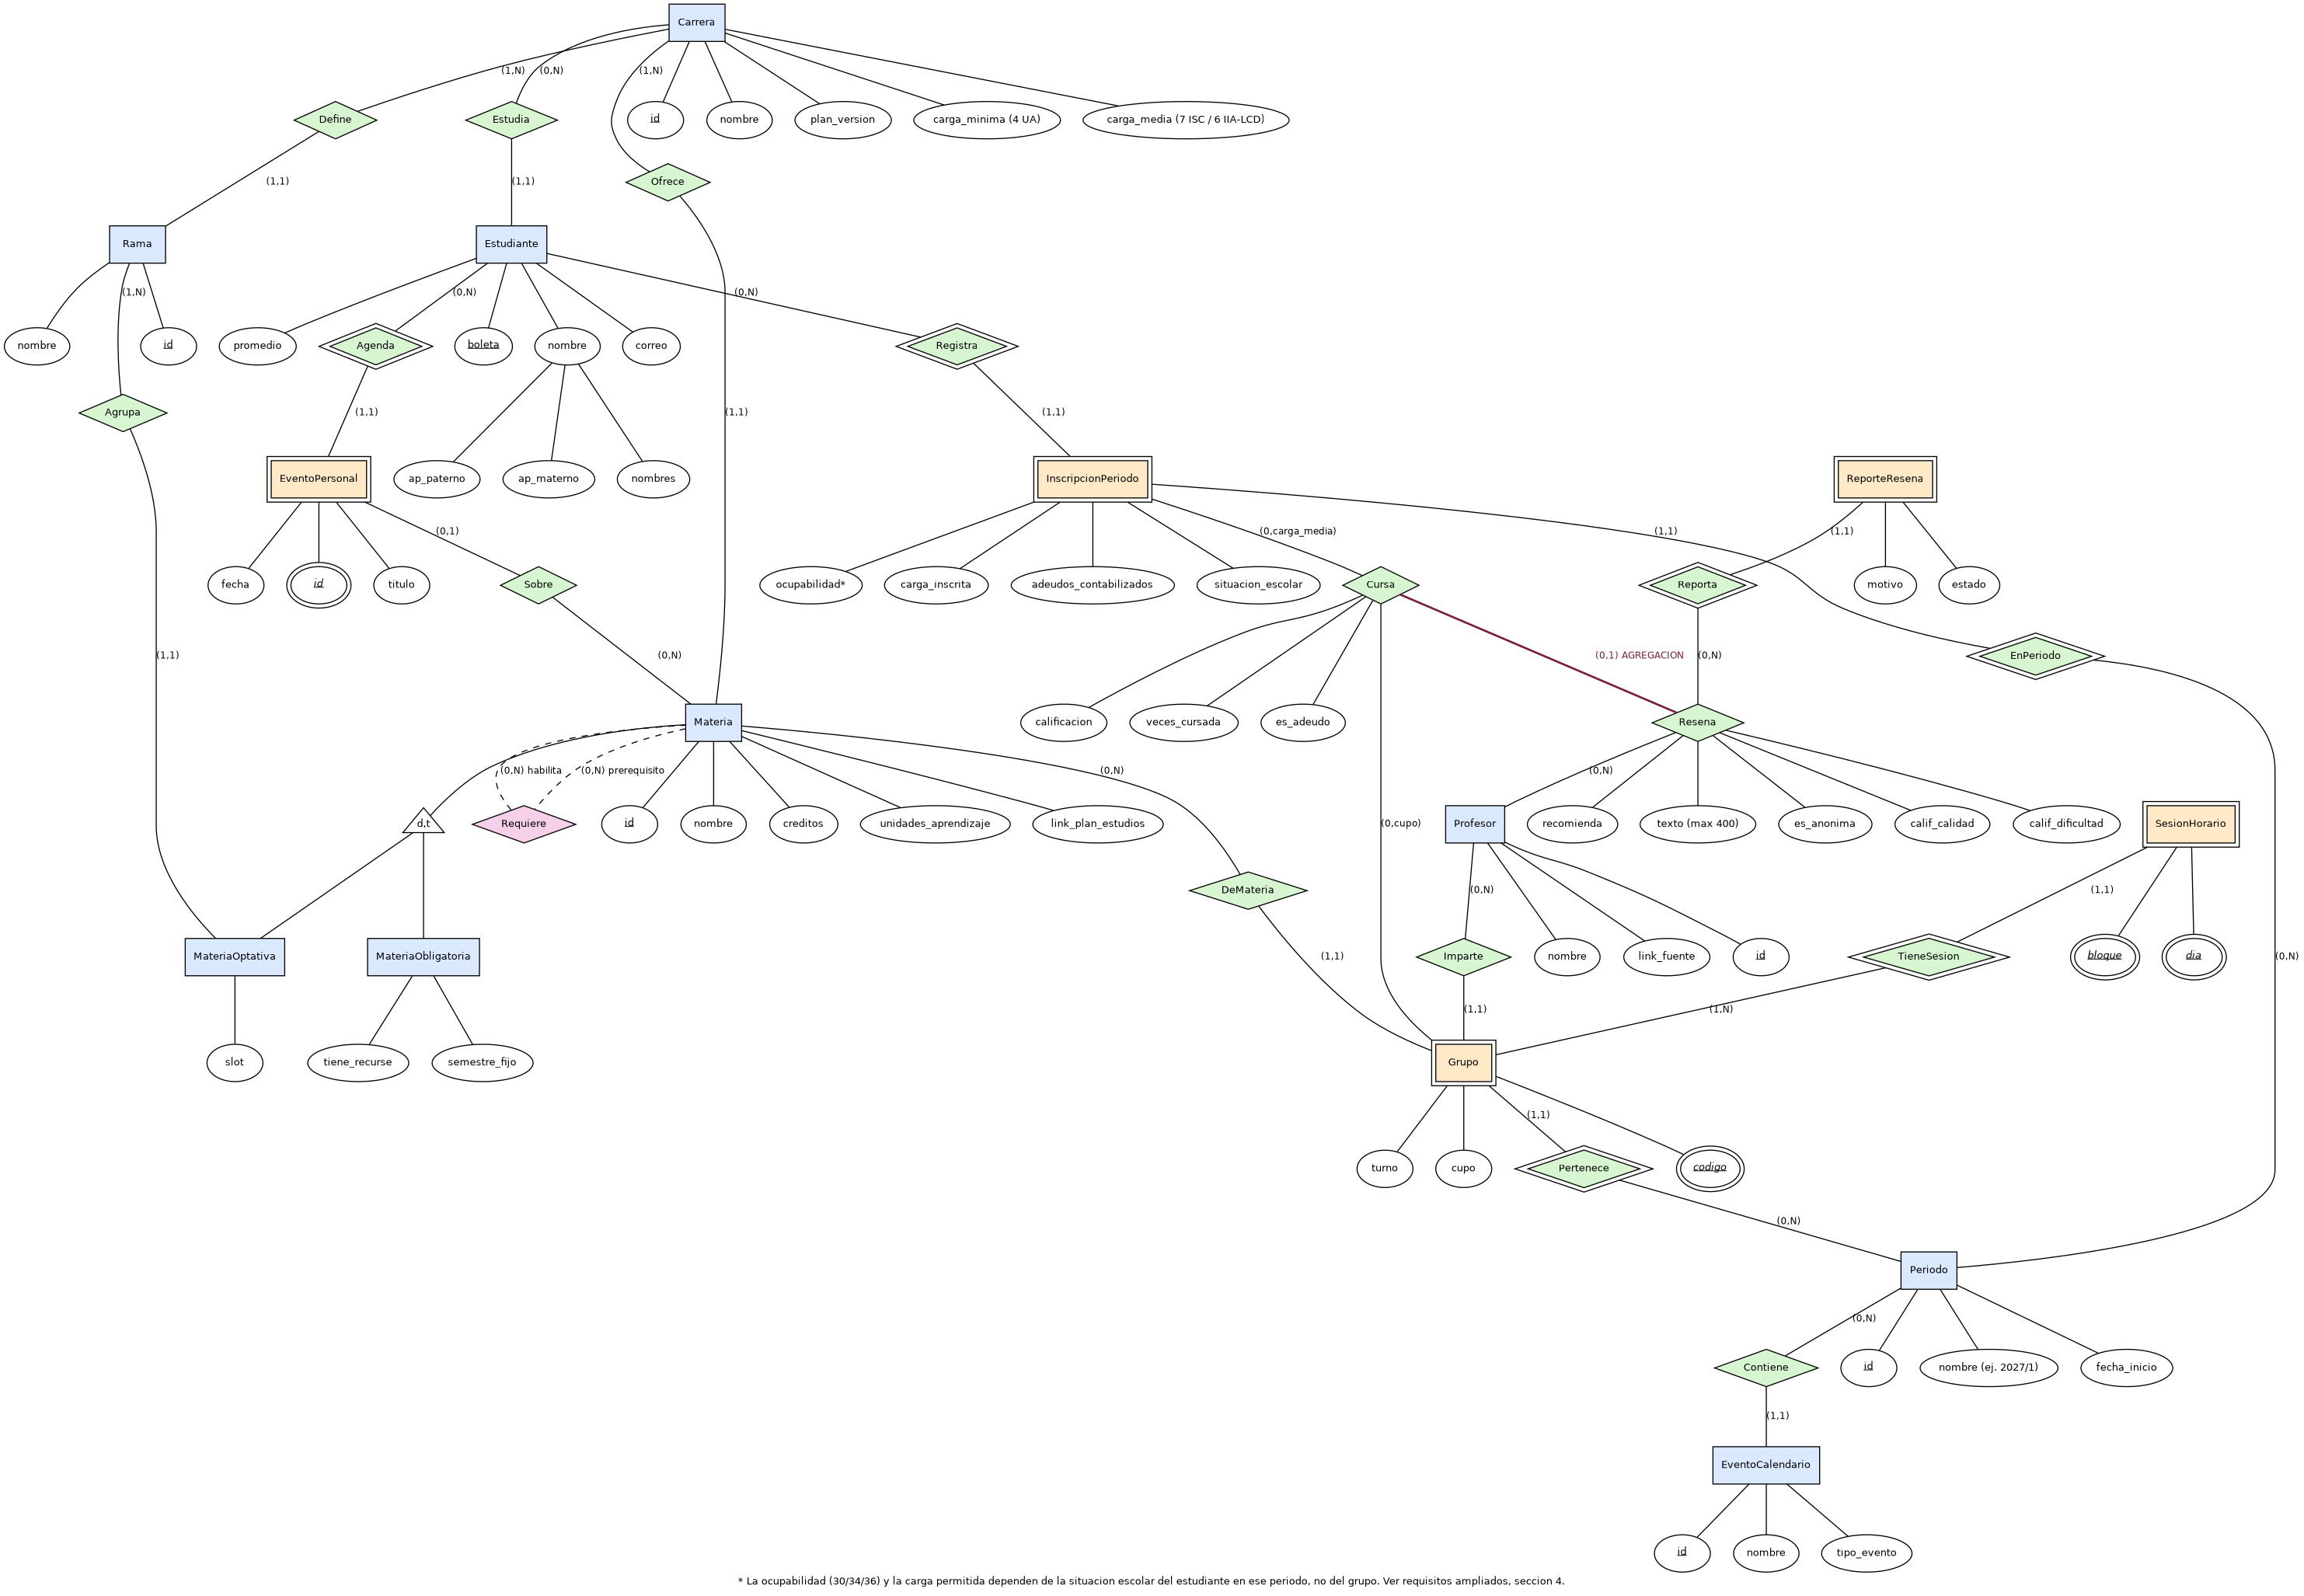
\includegraphics[width=\textwidth,keepaspectratio]{eer-chen.png}
\end{center}

\subsection{Notación Crow's Feet}

\begin{center}
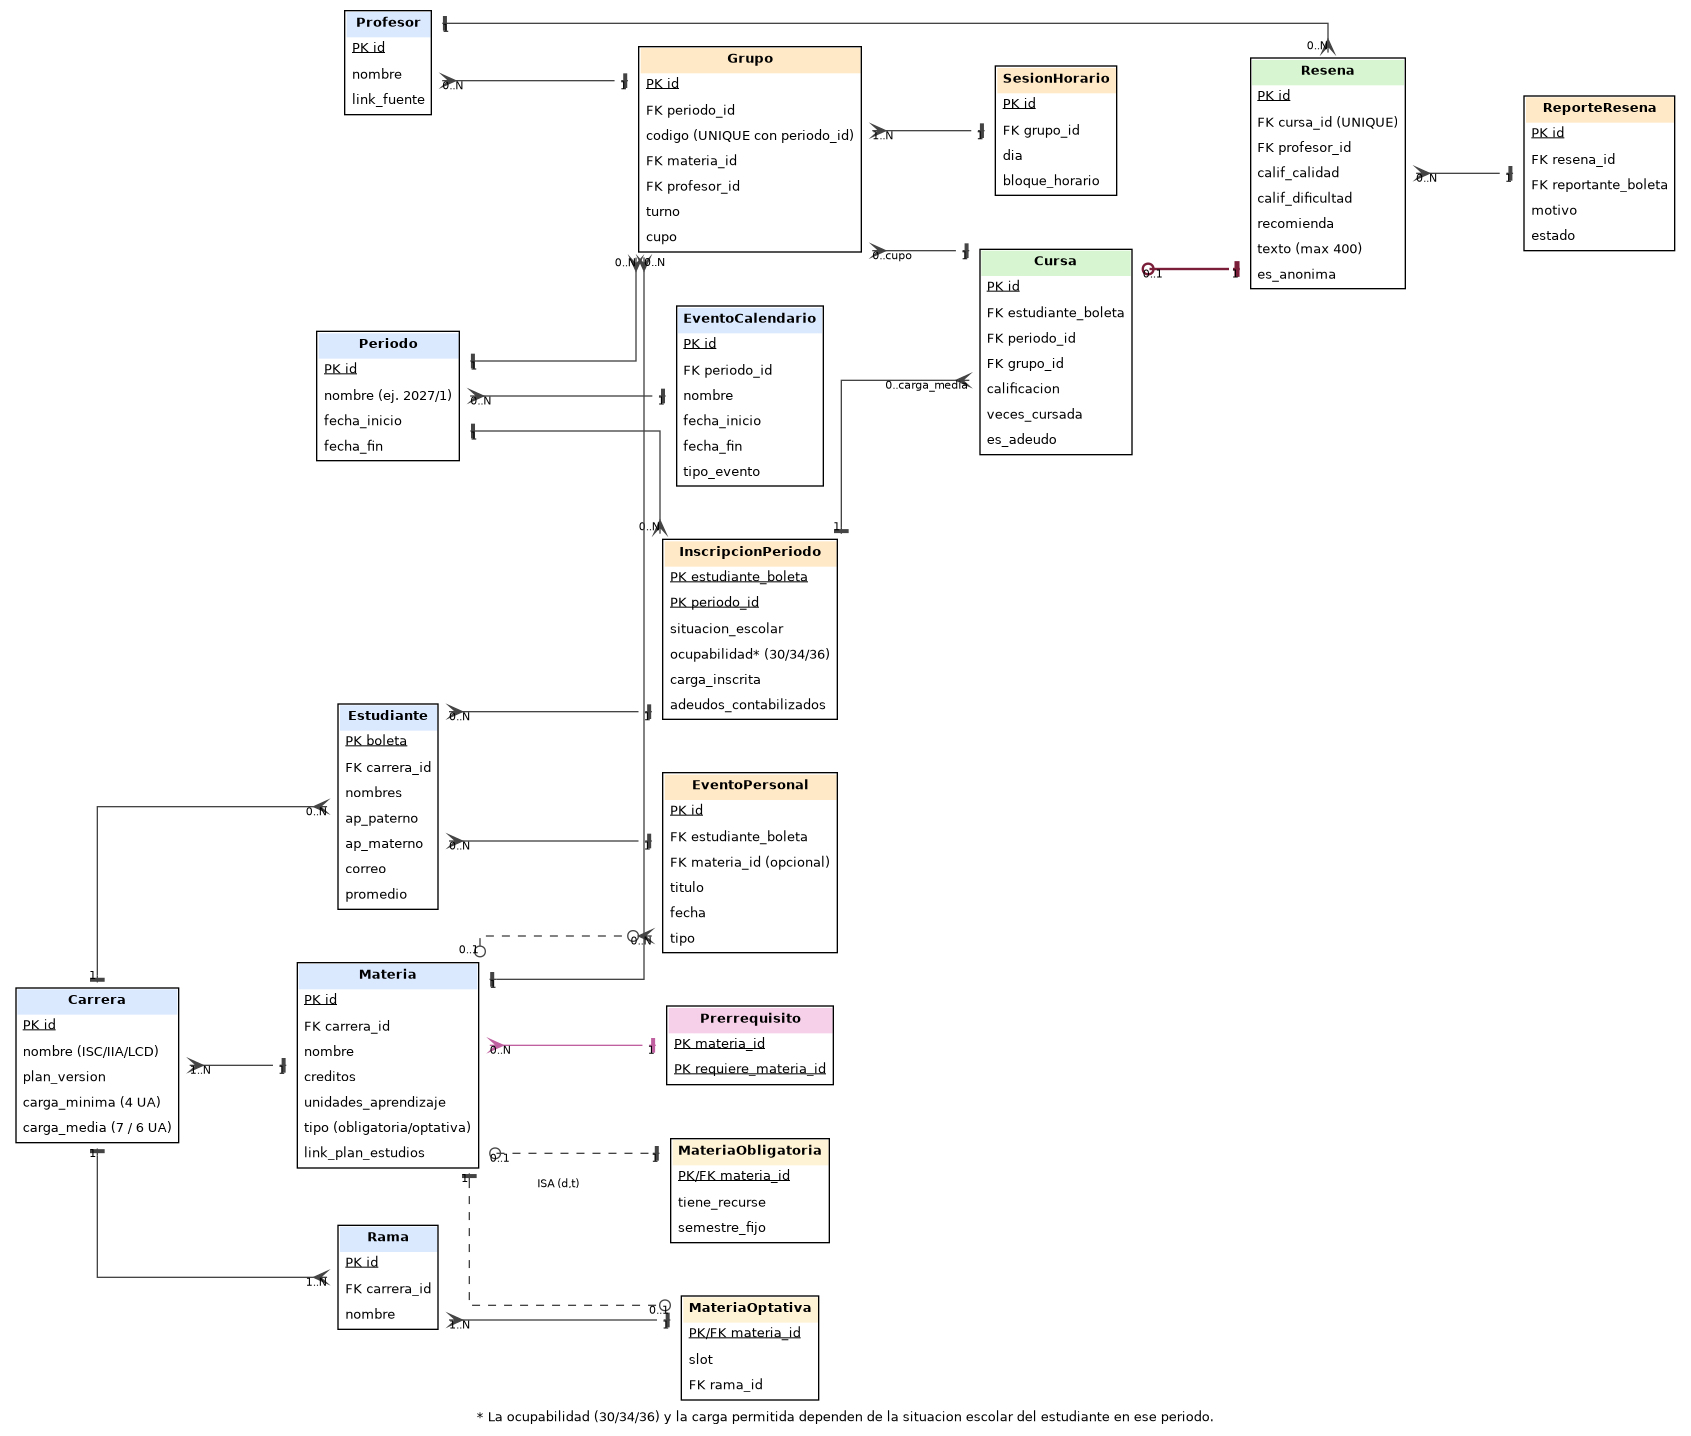
\includegraphics[height=0.75\textheight,keepaspectratio]{eer-crows-feet.png}
\end{center}

\section{Referencias}

\begin{itemize}[leftmargin=2em]
  \item[] Escuela Superior de Cómputo. (2020). \textit{Programa de estudios: Matemáticas Discretas, plan ISC-2020}. Instituto Politécnico Nacional. \url{https://www.escom.ipn.mx/docs/oferta/uaISC2020/matematicasDiscretas_ISC2020.pdf}

  \item[] Instituto Politécnico Nacional. (2026). \textit{Calendario académico 2026-2027, modalidad escolarizada}. Secretaría de Educación Pública.

  \item[] Instituto Politécnico Nacional. (s.f.). \textit{Sistema de Administración Escolar (SAES), Escuela Superior de Cómputo}. \url{https://www.saes.escom.ipn.mx/}
\end{itemize}

\end{document}
